\documentclass[12pt,reqno]{amsart}
\usepackage{fullpage}
\usepackage{amsfonts}
\usepackage{amssymb}
\usepackage{times}
\usepackage{graphicx}
\usepackage{hyperref}
\vfuzz=2pt

% some "funny lines" referred to later:
\newtheorem{thm}{Theorem}[section]
\newtheorem{cor}[thm]{Corollary}
\newtheorem{lem}[thm]{Lemma}
\newtheorem{prop}[thm]{Proposition}
\newtheorem{example}[thm]{Example}
\newtheorem{definition}[thm]{Definition}
{ \theoremstyle{remark}\newtheorem*{remark}{Remark} }


\newcommand{\tex}{{\tt .tex}}

%\newenvironment{definition}[1][Definition]{\begin{trivlist}
%\item[\hskip \labelsep {\bfseries #1}]}{\end{trivlist}}

\begin{document}

\title[Short version of title]{Reading Notes on \\ \small \emph{Automata Theory Language and Computation}}
% or if you want, simply \title{Title of the article}
\author{Jiecao Chen \\ \tiny jieca001@umn.edu }

\maketitle
\begin{abstract}
This will be a reading note on the book \textit{Introduction to Automata Theory Languages and Computation}. It consists of both the content from the book and my own thinking based on those content. 
\end{abstract}
\tableofcontents

\section{Automata: The Methods and the Madness}
\subsection{Why study Automata Theory}
This section serves to introduce the principal motivation and also outlines the major topics covered in book \cite{book1}.

\subsubsection{Introduction to Finite Automata}
Here are some examples that Finite Automata will be used
\begin{itemize}
	\item Software for designing and checking the behavior of digital circuits.
	\item The "lexical analyzer" of a typical compiler, that is, the compiler component that breaks the input text into logical units, such as identifiers, keywords, and punctuation.
	\item Software for scanning large bodies of text, such as collections of Web pages, to find occurrences of words, phrases, or other patterns.
	\item Software for verifying system of all types that have a finite number of distinct states, such as communications protocols or protocols for secure exchange of information.
\end{itemize}

\subsubsection{Structural Representations}
There are two important notations that are not automation-like, but play an important role in the study of automata and their applications.

\begin{itemize}
	\item \textit{Grammars} are useful models when designing software that processes data with a recursive structure. The "best-know" example is a "parser", the component of a compiler that deals with the recursively nested features of the typical programming language, such as expressions -- arithmetic, conditional, and so on. For instance, a grammatical rule like $E \Rightarrow E + E$ states that an expression can be formed by taking any two expressions and connecting them by a plus sign; this rule is a typical of how expressions of real programming language are formed. Context-free grammars may be covered later (which was first formulated by one of the best-known scholar, \textit{Avram Noam Chomsky}). 
	\item \textit{Regular Expressions} also denote the structure of data, especially text strings. The text described by \textit{regular expressions} is exactly same as what can be described by finite automata.
\end{itemize}

\subsubsection{Automata and Complexity}
Automata are essential for the study of the limits of computation. There are two important issues:
\begin{itemize}
	\item What can a computer do at all? This study is called "decidability", and the problems that can be solved by computer are called "decidable".
	\item What can a computer do efficiently? This study is called "intractability", and the problems that can be solved by a computer using no more time than some slowly growing function of the size of the input are called "tractable". Often, full polynomial functions are considered to be "slowly growing" while function that grow faster than than any polynomial are deemed to grow too fast.
\end{itemize}



\subsection{The Central Concepts of Automata Theory}
This section will give the definitions of most important terms that pervade the theory of automata.

\subsection{Alphabets}
An alphabet is a finite, nonempty set of symbols. Conventionally, we use the symbol $\Sigma$ for an alphabet. Common alphabets include:
\begin{itemize}
	\item $\Sigma = \{0,1\}$, the binary alphabet
	\item $\Sigma = \{a, b, \ldots, z\}$, the set of all lower-case letters.
	\item The set of all ASCII characters, or the set of all printable ASCII characters.
\end{itemize}

\subsubsection{Strings}
A \textit{string} (or sometimes \textit{word}) is a finite sequence of symbols chosen from some alphabet. For example, $01010$ is a string from the binary alphabet $\Sigma = \{0,1\}$.

\textbf{The Empty String}
The \textit{empty string} is the string with zero occurrences of symbols. This string is normally denoted as $\epsilon$.

\textbf{Length of a String}
Then \textit{length} of string $w$ Normally denoted as $|w|$. 

\textbf{Power of an Alphabet}
$\Sigma^k = \{w \big | |w| = k ~\mbox{and}~ w~ \mbox{is a string from} ~\Sigma \} $.

Here are several related concepts:
\begin{itemize}

	\item $\Sigma^* = \Sigma^0 \cup \Sigma^1 \cup \Sigma^2 \cup \ldots$

	\item $\Sigma^+ = \Sigma^1 \cup \Sigma^2 \cup \ldots$
\end{itemize}

\textbf{Concatenation of Strings}
Let $x$ and $y$ be strings, then $xy$ denotes the \textit{concatenation} of $x$ and $y$.

\textbf{Languages}
If $\Sigma$ is an alphabet, and $L \subseteq \Sigma^*$, then $L$ is a \textit{language over} $\Sigma$. 

\subsubsection{Problems}
If $\Sigma$ is an alphabet, and $L$ is a language over $\Sigma$, then the problem $L$ is:
\begin{quote}
	Give a string $w$ in $\Sigma^*$, decide whether or not $w$ is in $L$.
\end{quote}
It turns out that anything we more colloquially called a "problem" can be expressed as membership in a language.



\section{Finite Automata}
\subsection{Definition of a Deterministic Finite Automaton}
A \textit{deterministic finite automaton} consists of:
\begin{itemize}
	\item A finite set of states, often denoted $Q$
	\item A finite set of \textit{input symbols}, often denoted as $\Sigma$
	\item A \textit{transition function} that takes as arguments a state and an input symbol and returns a state. The function will commonly be denoted $\delta$. 
	\item A \textit{start state}, one of the states in $Q$
	\item A set of \textit{final} or accepting states $F$. The set is a subset of $Q$.
\end{itemize}	
A deterministic finite automaton will often be referred to by its acronym: DFA. The most succinct representation of a DFA is a listing of the five components above. In proofs we often talk about a DFA in "five-tuple" notation:
$$
	A = (Q, \Sigma, \delta, q_0, F)
$$
where $A$ is the name of the DFA, $Q$ is its set of states, $\Sigma$ its input symbols, $\delta: Q\times\Sigma \mapsto Q$ its transition function, $q_0$ its start state, and $F$ its set of accepting states.
A example:
\begin{example}
	$A = (\{q_0, q_1, q_3\}, \{0,1\}, \delta, q_0, \{q_1\})$
\end{example}
One thing should be mentioned is that the transition could also be extended to $\hat{\delta}:Q\times\Sigma^+\mapsto Q$, i.e. it takes a state and a string as input then gives a state as a output.

Following picture will be a informal illustration of a DFA.

\begin{center}
	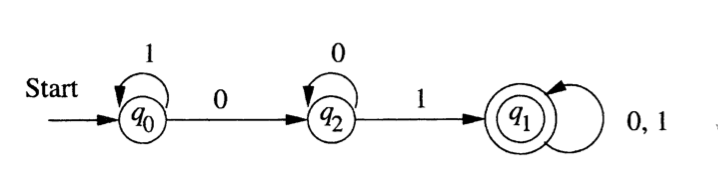
\includegraphics[width=0.7\textwidth]{example1}
	
	\textit{An example of a DFA}
\end{center}


\subsubsection{The Language of a DFA}
The \textit{language} of a DFA $A = (Q, \Sigma, \delta, q_0, F)$, denoted $L(A)$, is defined by:
$$
	L(A) = \{w | \hat{\delta}(q_0,w) ~\text{is in}~ F \}
$$

If $L$ is $L(A)$ for some DFA $A$, then we say $L$ is \textit{regular language}.

\subsubsection{Definition of Nondeterministic Finite Automata}
Let us introduce the formal notions associated with nondeterministic finite automamta. The differences between DFA's and NFA's will be pointed out as we do. An NFA is represented essentially like a DFA:
$$
	A = ( Q, \Sigma, \delta, q_0, F )
$$
Where:
\begin{itemize}
	\item $Q$ is a finite set of \textit{states}.
	\item $\Sigma$ is a finite set of \textit{input state}.
	\item $q_0$, a member of $Q$, is the \textit{start state}.
	\item $F$, a subset of $Q$, is the set of \textit{final} (or accepting) states.
\end{itemize}
 



\subsection{Nondeterministic Finite Automata}
A "nondeterministic" finite automaton (NFA) has the power to be in several states at once. This ability is often expressed as an ability to "guess" something about its input. For instance, when the automation is used to search for certain sequences of characters (e.g., keywords) in a long text string, it is helpful to "guess" that we are at the beginning of one of those strings and use a sequence of states to do nothing but check that string appears, character by character.

A informal example:

\begin{center}
	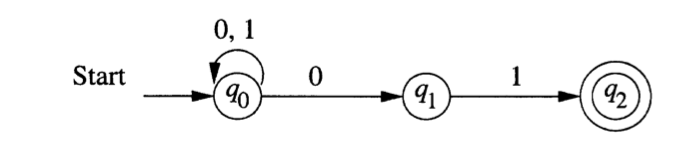
\includegraphics[width=0.7\textwidth]{NFA}
	
	\textit{An NFA accepting all strings that end in $01$}
\end{center}

\subsubsection{The Extended Transition Function}
We need to extend the transition function $\delta$ to $\hat{\delta}$ to make it has the ability to take a state and a string as an input and give a column of states as an output. Let's use INDUCTION to construct such functions.

\textbf{BASIS}: $\hat{\delta}(q,\epsilon) = \{q\}$

\textbf{INDUCTION}: Suppose $w$ is of the form $w=xa$, where $a$ is the final symbol of $w$ and $x$ is the rest of $w$. Also suppose that $\hat{\delta}(q,x) = \{p_1,p_2, \ldots, p_k \}.$ Let
$$
	\cup_{i=1}^k\delta(p_i,a) = \{r_1, r_2, \ldots, r_m \}
$$  

Then $\hat{\delta}(q,w) = \{r_1, r_2, \ldots, r_m \}$.

\subsubsection{The Language of an NFA}
Formally, if $A = (Q, \Sigma, \delta, q_0, F)$ is an NFA, then
$$
	L(A) = \{w | \hat{\delta}(q_0,w) \bigcap F \neq \emptyset \}
$$

\subsubsection{Equivalence of Deterministic and Nondeterministic Finite Automata}
Although there are many languages for which an NFA is easier to construct than a DFA, such as the language of strings that end in $01$, it is a surprising fact that \textbf{every language that can be described by some NFA can also be described by some DFA}, the proof involves a technique called \textit{subset construction} which constructs all subsets of the set of stats of the NFA.

\begin{thm}
	If $D = (Q_D, \Sigma, \delta_D, \{ q_0\}, F_D)$ is the DFA constructed from NFA $N = (Q_N, \Sigma, \delta_N, q_0, F_N)$ by the subset construction, then $L(D) = L(N).$ 
\end{thm}
Further, we have
\begin{thm}
	A language $L$ is accepted by some $DFA$ if and only if $L$ is accepted by some $NFA$.
\end{thm}

\subsection{Finite Automata With Epsilon-Transitions}
A $\epsilon-$NFA (or $\epsilon$-DFA) is an extended NFA such that  it also accepts $\epsilon$ as input of the transition function, i.e. the input set will be $\{\epsilon\}\cup \Sigma$.



\begin{thm}
	A language $L$ is accepted by some $\epsilon-$NFA if and only if $L$ is accepted by some DFA.
\end{thm}




\section{Regular Expressions and Languages}
"Regular Expression" are another type of language-defining notation, which may be thought of as a "programming language". It has various applications such as text-search application or compiler components. Regular expressions are closely related to nondeterministic finite automata and can be thought of as a "user-friendly" alternative to the NFA notation for describing software components.

\subsection{Regular Expressions}
"Regular Expressions" is regarded as a kind of algebraic description of language, comparing with the machine-like description: NFA and DFA.
We shall find that regular expressions can define exactly the same languages that the various forms of automata describe: the regular languages. However, regular expressions offer something that automata do not: a declarative way to express the strings we want to accept. Thus, regular expressions serve as the input language for many systems that process strings. Examples:
	\begin{itemize}
	\item Search command such as UNIX \textbf{grep}. Different search engines convert the regular expressions to DFA or NFA, and simulate that automaton on the file being searched.
	\item Lexical-analyzer, such as \textbf{Lex} or \textbf{Flex}. Both are extremely useful to construct compilers.
	\item As discussed in book \cite{book2}, \textit{Mathematica} is a pattern-matching system, in some sense, the \textit{Mathematica Programming Language} could be considered as an extended version of \textit{regular expressions}.
	\end{itemize}
	
\subsubsection{The Operators of Regular Expressions}
Regular expressions denote languages. For example, \textbf{$01^*+10^*$} denotes the language consisting of all strings that are either a single $0$ followed by any number of $1$'s or a single $1$ followed by any number of $0$'s. Here are the operations:
\begin{itemize}
	\item The \textit{union} of two languages $L$ and $M$, denoted $L\cup M$
	\item The \textit{concatenation} (called \textit{dot}) of language $L$ and $M$ is the set of strings that can be formed by taking any string in $L$ and concatenating it with any string in M, denoted $L.M$ or just $LM$.	
	\item The \textit{closure} (or \textit{star}, or \textit{Kleene closure}) of a language $L$ is denoted $L^*$ and represents the set of those strings that can be formed by taking any number of strings from $L$, possibly with repetitions and concatenating all of them. Formally, $L^* = \cup_{i\geq 0}L^i$ where $L^0 = \{ \epsilon\}$, $L^1 = L$, for $i > 1$ is $L^i = LL\ldots L$ (the concatenation of $i$ copies of $L$) .
	
\end{itemize}


\subsubsection{Building Regular Expressions}
The algebra of regular expressions use constants and variables that denote languages together with three operators described - union, dot and star. Regular Expression can be described recursively. For each regular expression $E$, we describe the language it represents, which we denote $L(E)$.

\textbf{BASIS}: The basis consist of three parts:
\begin{itemize}
	\item The constants $\epsilon$ and $\emptyset$ are regular expressions, denote the language $\{\epsilon\}$ and $\emptyset$, that is, $L(\epsilon) = \{\epsilon\}$, and $L(\emptyset) = \emptyset$.
	\item If $a$ is any symbol, then $\textbf{a}$ is a regular expression. This expression denotes the language $\{a\}$. That is $L(\textbf{a}) = \{ a \}$. Note that we use boldface font to denote an expression corresponding to a symbol, i.e. \textbf{$a$} refers to $a$.
	\item A variable, usually capitalized and italic such as \textit{\textbf{L}}, is a variable, representing any language.
\end{itemize}

\textbf{INDUCTION}:There are four parts to the inductive step, one for each of the three operators and one for the introduction of parentheses.
\begin{itemize}
	\item If $E$ and $F$ are regular expressions, then $E+F$ is a regular expression denoting the union of $L(E)$ and $L(F)$. That is, $L(E+F)=L(E)\cup L(F)$.
	\item If $E$ and $F$ are regular expressions, then $EF$ is a regular expression. $L(EF) = L(E)L(F)$
	\item If $E$ is a regular expression, then $E^*$ is a regular expression, denoting the closure of $L(E)$. $L(E) = (L(E))^*$
	\item If $E$ is a regular expression, then $(E)$ denote the same language as $E$
\end{itemize}
\textbf{IMPORTANT:} Strictly speaking, a regular expression $E$ is just an expression, not a language, but we sometime use this symbol to represent the language $L(E)$. It is common usage to refer to say "$E$" when we really mean "$L(E)$".	 

\subsubsection{Precedence of Regular-Expression Operators}
\textbf{Star} is higher than \textbf{dot}, and dot is higher than \textbf{union}. Of course, parentheses can in someway change the order.

\subsection{Finite Automata and Regular Expressions}
Here are some facts:
\begin{itemize}
	\item Every language defined by one of these automata is also definted by a regular expression. For the proof, we can assume the language is accepted by some DFA.
	\item Every language definted by a regular expression is definted by one of these automata. For this part of th proof, the easiest is to show that there is a NFA with $\epsilon-$transitions accepting the same language. The following figure shows all the equivalences we mentioned:
	
\begin{center}
	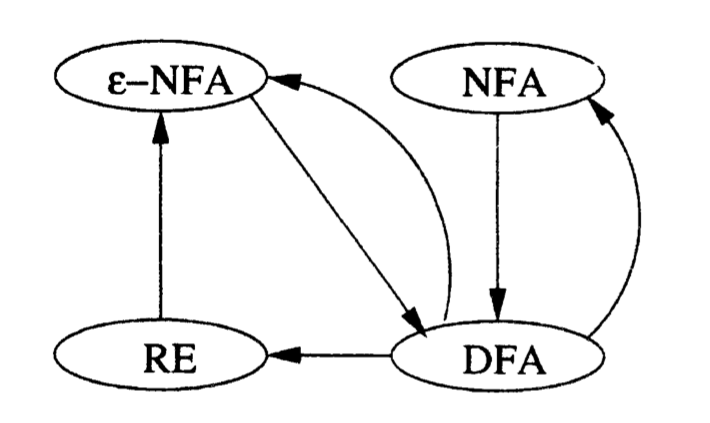
\includegraphics[width=0.5\textwidth]{equal}
		
	\textit{The equivalence of four different notations for regular languages}
\end{center}
	
\end{itemize}


\begin{thebibliography}{99} % don't worry about the 99

\bibitem{book1}
Hopcroft, John E. \textbf{\textit{Introduction to Automata Theory, Languages, and Computation}}, 3/E. Pearson Education India, 2008.

\bibitem{paper1}
Thompson, Ken. \textbf{\textit{Programming Techniques: Regular expression search algorithm.}} Communications of the ACM 11.6 (1968): 419-422.

\bibitem{paper2}
Wadler, Philip. \textbf{\textit{The essence of functional programming}}. Proceedings of the 19th ACM SIGPLAN-SIGACT symposium on Principles of programming languages. ACM, 1992.


\bibitem{book2}
Wolfram, Stephen. \textbf{\textit{The Mathematica Book}}, Version 4. Cambridge university press, 1999.

\end{thebibliography}

\end{document}
